% !TEX TS-program = xelatex
\documentclass[12pt]{beamer}
\usetheme{metropolis}
\usepackage{tabularx}
\usepackage{changepage}
\usepackage{float}
\usepackage{ragged2e}
\usepackage{amsmath}
\usepackage{graphicx}
\usepackage{appendix}
\usepackage{bbm}
\usepackage{amsmath}
\usepackage{algorithm}
\usepackage{algpseudocode}
\usepackage[round]{natbib}   % omit 'round' option if you prefer square brackets
\bibliographystyle{aer}
\usepackage{setspace}


% \usepackage{xeCJK}
\setCJKmainfont{regular}[
    Path="fonts/simplified_chinese/noto_serif/",
    BoldFont=bold.otf
]
\xeCJKDeclareSubCJKBlock{Hangul}{"1100 -> "11FF, "3130 -> "318F, "A960 -> "A97F, "AC00 -> "D7AF, "D7B0 -> "D7FF}
\setCJKmainfont{regular}[
    Hangul,
    Path="fonts/korean/noto_serif/",
    BoldFont=bold.otf
]

\xeCJKDeclareSubCJKBlock{Kana}{"3040 -> "309F, "30A0 -> "30FF, "31F0 -> "31FF, "1B000 -> "1B0FF}
\setCJKmainfont{regular}[
    Kana,
    Path="fonts/japanese/noto_serif/",
    BoldFont=bold.otf
]



\title{\huge{Introduction To Louvain Method}}
\author{Hsiu-Hsuan Yeh}
\date{2024-05-28}


\begin{document}
\maketitle


\begin{frame}{Resources}
\begin{itemize}
    \item \cite{leskovec2021communities}
\end{itemize}
\end{frame}


\begin{frame}{Outline}
\tableofcontents
\end{frame}


\section{Modularity}
\subsection{What Is Modularity?}
\begin{frame}{Overview}
\cite{clauset2004finding} states that modularity measures when the division is
a good one, in the sense that there are many edges within communities and only
a few between them.

Modularity-based method including \cite{blondel2008fast} evaluates the division by
considering a hypothetical model. Given the division
C, if the density of the connection within each community is
higher than the hypothetical model, then C is somehow a relatively good division.
\end{frame}


\begin{frame}{Overview}
\centering
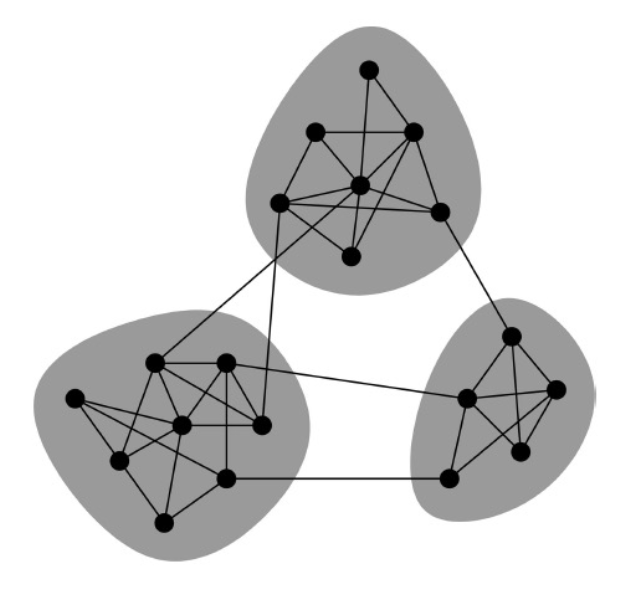
\includegraphics[width=8cm]{img/img1.png}
% \caption{}
\end{frame}


\begin{frame}{Formula}
$$
Q(C) = \frac{1}{2m}\Sigma_{i, j} (A_{ij}-\frac{k_ik_j}{2m})\delta(c_i, c_j)
$$
\begin{itemize}
    \item $C$: the structure of the division, communities
    \item $A_{i, j}$: edge weight, can be a binary or real number
    \item $k_i$: $\Sigma_j A_{i, j}$, the total edge weight of a node i
    \item $2m$: $\Sigma_{i, j}A_{i, j}$, the total edge weight of a graph
    \item $\delta$: indicating wheter the node i and j are in the same community
\end{itemize}
\end{frame}


\subsection{Hypothetical Model: Expected Edge Weight}
\begin{frame}{Hypothetical Model: Expected Edge Weight}
$$
Q(C) = \frac{1}{2m}\Sigma_{i, j} (A_{ij}-\frac{k_ik_j}{2m})\delta(c_i, c_j)
$$
\begin{itemize}
    \item  $\frac{k_ik_j}{2m}$ is the expected edge weight for both node i and j
    \item assume each node remains its edge weight and the connection between nodes is random

    \begin{itemize}
            \item view $2m$ as the number of all “available ports”
            \item for node i, the edge weight assoicated to node j follows
                the binomial distribution, Binomial($k_i, \frac{k_j}{2m}$)
            \item the expected edge weight,
                $E(\text{edge weight}_{i, j}) = k_i\frac{k_j}{2m}$
    \end{itemize}
\end{itemize}
\end{frame}


\begin{frame}{Hypothetical Model: Expected Edge Weight}
\centering
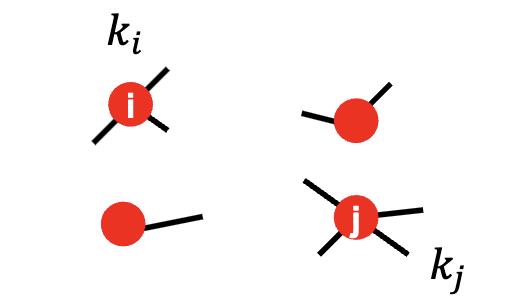
\includegraphics[width=11cm]{img/img2.png}
% \caption{}
\end{frame}


\section{Alogrithm}
\begin{frame}{Algorithm}
\centering
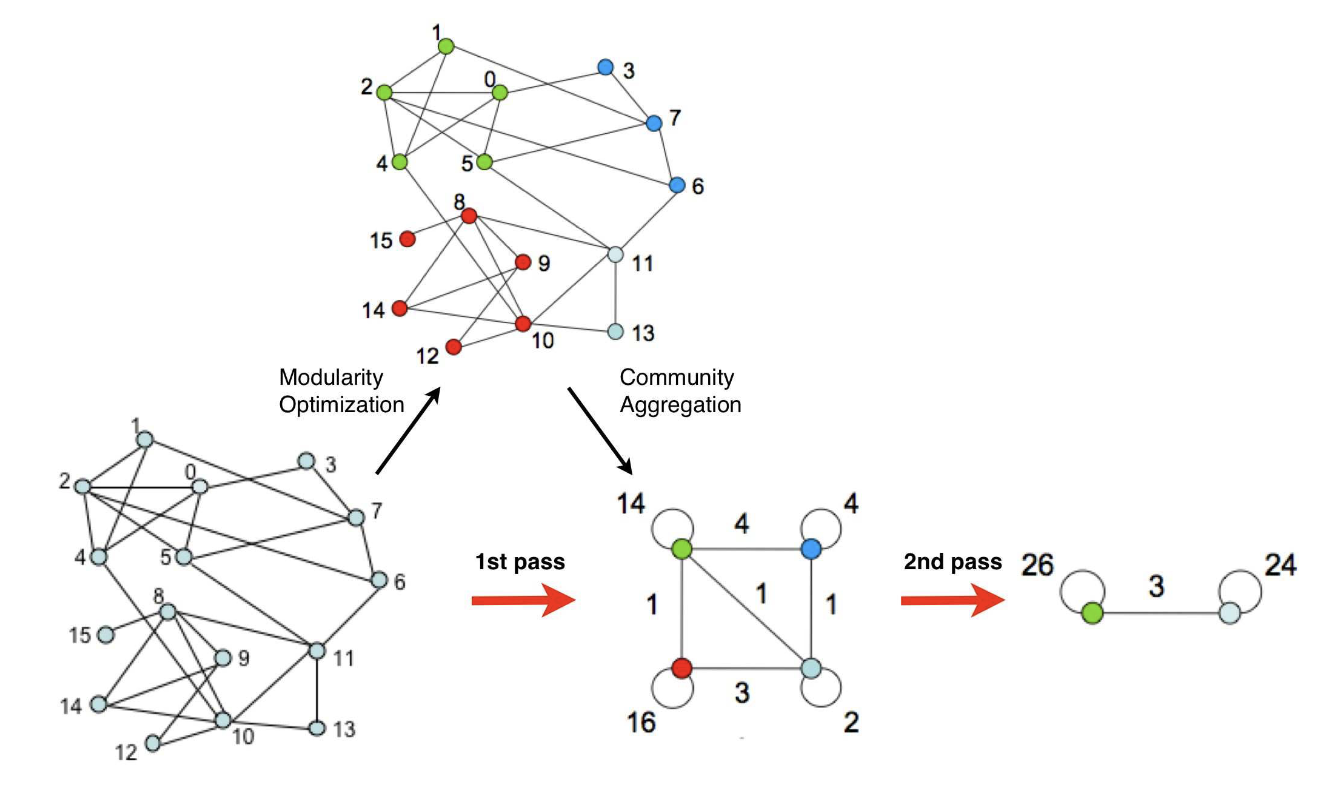
\includegraphics[width=11cm]{img/img3.png}
% \caption{}
\end{frame}


\begin{frame}{Algorithm}
Modularity Optimization
\begin{itemize}
    \item initialize each node in its own community
    \item for each node $i \in V$, compute the gain($\Delta Q$) in modularity by moving $i$ to the community of each of its neighbors
    \item the node i will then be placed in the coummunity which has the hightest
        positive modularity gain($\Delta Q$)
\end{itemize}

$\Delta Q = \left[ \frac{\sum_{in} + k_{i,in}}{2m} - \left( \frac{\sum_{tot} + k_i}{2m} \right)^2 \right] - \left[ \frac{\sum_{in}}{2m} - \left( \frac{\sum_{tot}}{2m} \right)^2 - \left( \frac{k_i}{2m} \right)^2 \right]$
\vspace{0.3cm}

Notice taht this is the change in Q when moving node i to a community. The
change in Q when moving i out of a coummunity is similar.
\end{frame}


\subsection{Revision Of Modularity Formula}
\begin{frame}{Revision Of Modularity Formula}
% \Large
\begin{align*}
Q(C)
    &= \frac{1}{2m}\Sigma_{i, j} (A_{i, j} - \frac{k_ik_j}{2m})\delta(c_i, c_j) \\
    &= \Sigma_{c\in C}\frac{\Sigma_{i, j\in c}A_{i, j}}{2m} - \frac{\Sigma_{i\in c}k_i\Sigma_{j\in c}k_j}{4m^2} \\
    &= \Sigma_{c\in C} \frac{\Sigma_{in,  c}}{2m} - \frac{\Sigma_{tot, c}\Sigma_{tot, c}}{4m^2} \\
    &= \Sigma_{c\in C} \underbrace{\frac{\Sigma_{in, c}}{2m}}_{\text{edge weight within $c$}}
        - ( \underbrace{\frac{\Sigma_{tot, c}}{2m}}_{\text{total edge weight of $c$}})^2
\end{align*}
\end{frame}


\begin{frame}{Some Notations}
\centering
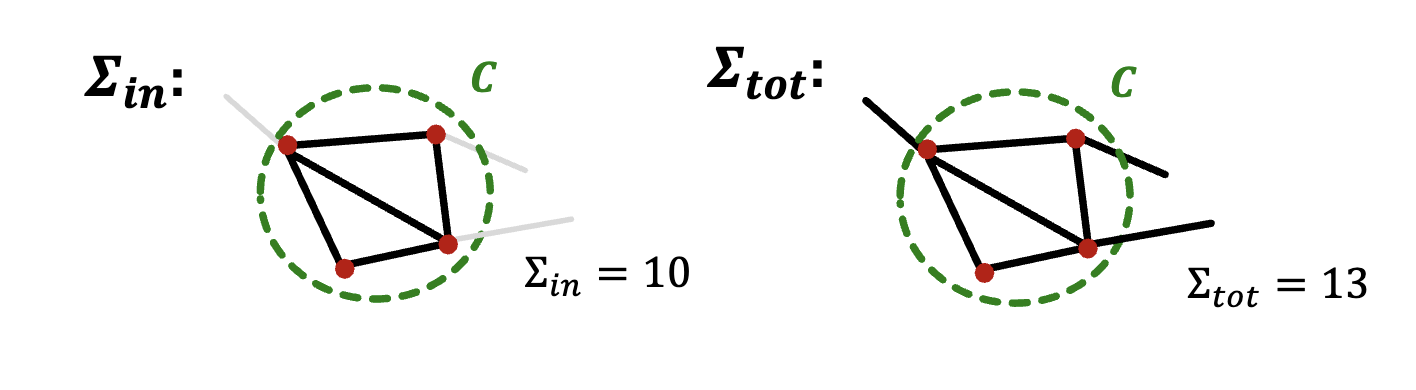
\includegraphics[width=11cm]{img/img4.png}
% \caption{}
\begin{itemize}
    \item $\Sigma_{in, c} = \Sigma_{i, j\in c}A_{i, j}$
    \item $\Sigma_{tot, c} = \Sigma_{i\in c}k_i = \Sigma_{i\in c}\Sigma_{j}A_{i, j}$
\end{itemize}
\end{frame}


\begin{frame}{More Notaions}
Considering a node i moving from community c to c’, there are two types of edge weights related to i.
\begin{itemize}
    \item $k_i = k_{i, c'} + k_{i, c}$
    \item associated to community c’: $k_{i, c'}$
    \item associated to community c: $k_{i, c}$
\end{itemize}
What we want to know is the change in modularity, $\Delta Q(C)$ for node i
moving from $c$ to $c'$. It consists of two components: moving into $c'$ and
moving out of $c$.

$\Delta Q(C) = \Delta Q(c') + \Delta Q(c)$
\end{frame}


\begin{frame}{Change In Modularity}
\centering
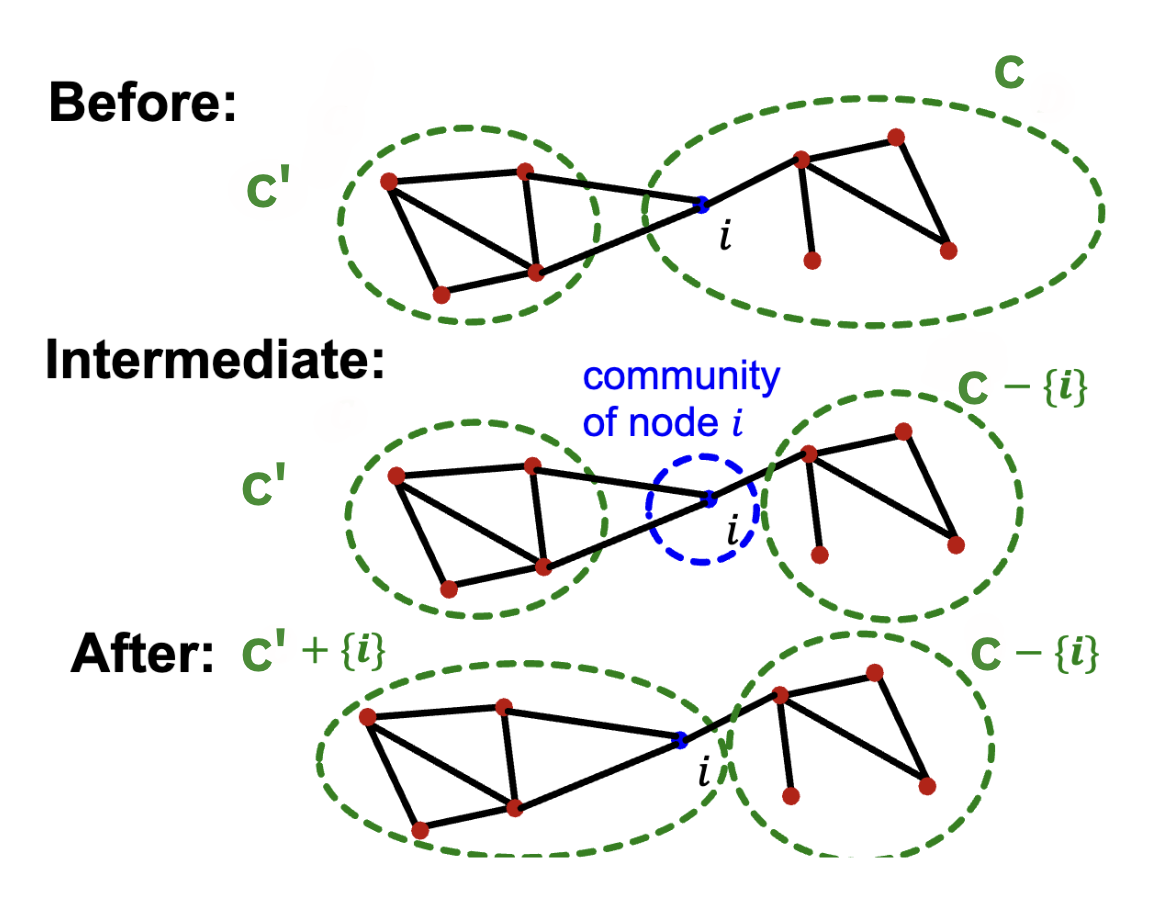
\includegraphics[width=10cm]{img/img5.png}
% \caption{}
\end{frame}


\subsection{Modularity Gain For Moving Into $c'$}
\begin{frame}{Moving Into $c'$}
\begin{itemize}
    \item $\Delta Q(c') = Q_{i\to c'}(c') - ( Q(c') + Q(i))$
    \item $Q(c')$: modularity of $c'$ before merging with node i
    \begin{itemize}
        \Large
        \item $\frac{\Sigma_{in, c'}}{2m} - (\frac{\Sigma_{tot, c'}}{2m})^2$
    \end{itemize}
    \item $Q(i)$: modularity of a community with a unique member i
    \begin{itemize}
        \Large
        \item $0-(\frac{k_i}{2m})^2 = - (\frac{k_i}{2m})^2$
    \end{itemize}
    \item $Q_{i\to c'}(c')$: modularity of $c'$ after merging with node i
    \begin{itemize}
        \Large
        \item $\frac{\Sigma_{in, c'}+2k_{i, c'}}{2m} - (\frac{\Sigma_{tot, c'}+k_i}{2m})^2$
    \end{itemize}
\end{itemize}
\end{frame}


\begin{frame}{Moving Into $c'$}
\begin{align*}
\Delta Q(c')
    &= Q_{i\to c'}(c') - ( Q(c') + Q(i)) \\
    &= \underbrace{\frac{\Sigma_{in, c'}+2k_{i, c'}}{2m} - (\frac{\Sigma_{tot, c'}+k_i}{2m})^2}_{Q_{i\to c'(c')}} \\
        &- [ \underbrace{\frac{\Sigma_{in, c'}}{2m} - (\frac{\Sigma_{tot, c'}}{2m})^2}_{Q(c')} \underbrace{- (\frac{k_i}{2m})^2}_{Q(i)} ] \\
    &= \frac{2k_{i, c'}}{2m} - \frac{2k_i\Sigma_{tot, c'}}{4m^2}
\end{align*}
\end{frame}


\subsection{Modularity Gain For Moving Out of $c$}
\begin{frame}{Moving Out of $c$}
\begin{itemize}
    \item $\Delta Q(c) = (Q_{c\to i}(c)+Q(i)) -  Q(c)$
    \item $Q(c)$: modularity of $c$ before node i moving out
    \begin{itemize}
        \Large
        \item $\frac{\Sigma_{in, c}}{2m} - (\frac{\Sigma_{tot, c}}{2m})^2$
    \end{itemize}
\item $Q_{c\to i}(c)$: modularity of $c$ after node i moving out
    \begin{itemize}
        \Large
        \item $\frac{\Sigma_{in, c} - 2k_{i, c}}{2m} - (\frac{\Sigma_{tot, c}-k_i}{2m})^2$
    \end{itemize}
\end{itemize}
\end{frame}

\begin{frame}{Moving Out of $c$}
\begin{align*}
\Delta Q(c)
    &= (Q_{c\to i}(c)+Q(i)) -  Q(c) \\
    &= [ \underbrace{\frac{\Sigma_{in, c} - 2k_{i, c}}{2m} - (\frac{\Sigma_{tot, c}-k_i}{2m})^2}_{Q_{c\to i(c)}} \underbrace{- (\frac{k_i}{2m})^2}_{Q(i)} ] \\
        &-  [ \underbrace{\frac{\Sigma_{in, c}}{2m} - (\frac{\Sigma_{tot, c}}{2m})^2}_{Q(c)} ] \\
        &= \frac{-2k_{i, c}}{2m} + \frac{2k_i\Sigma_{tot, c}}{4m^2} - 2(\frac{k_i}{2m})^2
\end{align*}
\end{frame}


\subsection{The intuition for Positive Modularity Gain Movement}
\begin{frame}{Modularity Gain}
\begin{align*}
\Delta Q(C)
    &= \Delta Q(c') + \Delta Q(c) \\
    &= \underbrace{\frac{2k_{i, c'}}{2m} - \frac{2k_i\Sigma_{tot, c'}}{4m^2}}_{\Delta Q(c')}
        + \underbrace{\frac{-2k_{i, c}}{2m} + \frac{2k_i\Sigma_{tot, c}}{4m^2} - 2(\frac{k_i}{2m})^2}_{\Delta Q(c)} \\
    &= \frac{2(k_{i, c'}-k_{i, c})}{2m} + \frac{2k_i((\Sigma_{tot, c} - k_i) - \Sigma_{tot, c'})}{4m^2}
\end{align*}

The intuition for positive modularity gain movement:
\begin{itemize}
    \item for node i, there are more connection in community $c'$ comapred to $c$, $k_{i, c'} > k_{i, c}$
    \item the size of c' is smaller than c, $\Sigma_{tot, c} - k_i > \Sigma_{tot, c'}$
\end{itemize}
\end{frame}


\subsection{Pros and Cons}
\begin{frame}{Pros and Cons}
Pros
\begin{itemize}
    \item comprehensive
    \item efficient - the height of dendrogram is usually short
\end{itemize}
Cons
\begin{itemize}
    \item high extra-space complexity: $O(|V|^2)$
    \item local optimization
    \item potential instability - the order of nodes for modularity optimization matters
\end{itemize}
\end{frame}


\begin{frame}{Application to large networks}
\centering
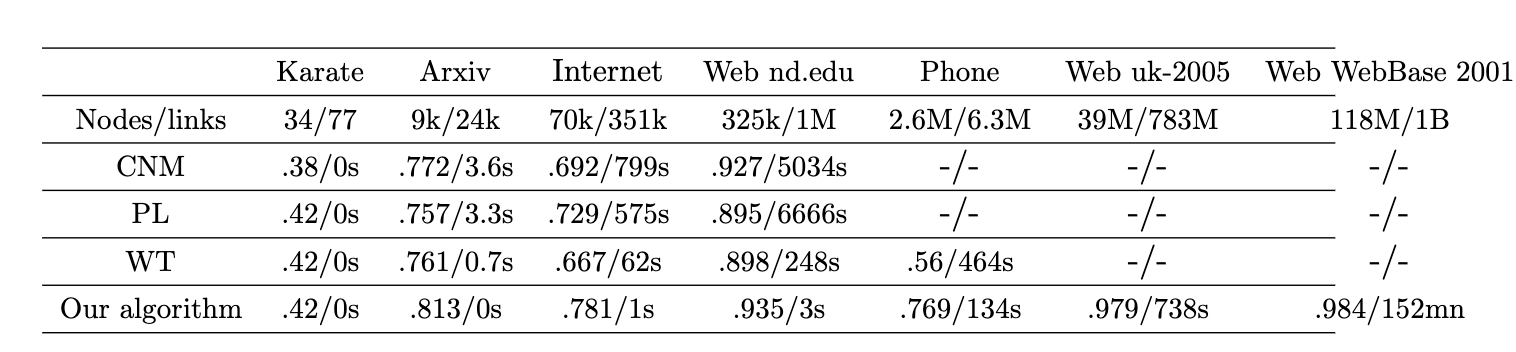
\includegraphics[width=11cm]{img/img6.png}
% \caption{}
\end{frame}


\section{References}


\begin{frame}[allowframebreaks]{}
\renewcommand{\section}[2]{}%
\bibliography{main.bib}
\end{frame}


\end{document}
